% Appendix B

% variables
\newcommand{\appdirb}{appendices/plots/appendixB}

\chapter{Physics tool} % Main appendix title

\label{AppendixB} % For referencing this appendix elsewhere, use \ref{AppendixB}

\section{Synchrotron radiation}
\label{appB:sec:sr}

Synchrotron radiation is the known phenomenon based on the basic principle of the electrodynamics, which state that an accelerated charged particle always radiates electromagnetic waves. In particular synchrotron radiation describes the energy emitted by a charged particle in a circular motion. This phenomena was already investigated theoretically at the beginning of the 20th century and was later first observed and experimentally studied at the General electric 70 MeV synchrotron from which it gets its name \cite{synchrotron-radiation}. \\
This type of radiation is well known thank to the advent of modern circular acceleration, where it is so strong that it can even be observed for heavy particles, like for instance protons. \\
The experiment aims to use such a radiation to tag the incoming particles in order to distinguish between the electron primaries and the background given by hadron and muons. A small review on this effect, which will underline the important properties exploited for the experiment,will be presented.


\subsection{Power emitted}
The first result about the power radiated by an accelerated non-relativistic particle was obtained by Larmor:

\begin{equation}
S = \frac{e^2}{6 \pi \epsilon_0 m_0^2 c^3}\left(\frac{dp}{dt}\right)^2
\label{eqn:radiated-power}
\end{equation}

The angular distribution can be calculated similarly to be:

\begin{equation}
\frac{dS}{d\Omega} = \frac{e^2}{6 \pi \epsilon_0 m_0^2 c^3}\left(\frac{dp}{dt}\right)^2\sin^2\Theta
\label{eqn:angular-dist}
\end{equation}

If we insert the number in the two previous equation it results that the power irradiated for a particle in the classical approximation is negligible even for particles as light as the electrons. \par 

The situation changes as we try to find a Lorentz-invariant form of the equation by applying the following transformation:
\begin{eqnarray}
dt \longrightarrow d\tau=\frac{1}{\gamma}dt \qquad
\gamma = \frac{1}{\sqrt{1-\beta^2}} \qquad \beta=\frac{v}{c}
\label{time_trans}
\end{eqnarray}

\begin{equation}
\left(\frac{dP_{\mu}}{d\tau}\right)^2 \longrightarrow \left(\frac{dp}{dt}\right)^2 - \frac{1}{c^2}\left(\frac{dE}{d\tau}\right)^2
\label{momentum-trans}
\end{equation}

If we put these expressions in Eq.\ref{eqn:radiated-power} we get a correspondent relativistic expression:
\begin{equation}
S = \frac{e^2c}{6\pi \epsilon_0}\frac{1}{(m_0c^2)^2 }\left[\left(\frac{dp}{dt}\right)^2 - \frac{1}{c^2}\left(\frac{dE}{d\tau}\right)\right]
\label{eqn:rel-power}
\end{equation}

The acceleration will strongly depend on the angle between the particle velocity and the acceleration as the time derivate of the impulse suggests. We will now concentrate on the extreme case where $dv/dt \perp v$ since it is our case of interest. It is possible, however, to derive the other extreme case $dv/dt|| v$ and verify that there is no difference from the classical one. \par

If we assume the particle to follow a circular motion (i.e $F \perp v$) we can conclude that the energy of the particle do not change during the motion. This already drops out the time-derivative of the energy from Eq.\ref{eqn:rel-power}. After that we can express the momentum of the particle as:
\[\frac{dp}{dt} =p\omega = p \frac{v}{R}\]
where R is the bending radius of the trajectory. We can further simplify the expression assuming $E=pc$, which is true for particle at high enough energy and it is certainly true for our experiment where the electrons have an energy of 100 GeV. After we express the momentum and velocity using these last approximation we get the result of:
\begin{equation}
S = \frac{e^2c}{6\pi \epsilon_0}\frac{1}{(m_0c^2)^4 }\frac{E^4}{R^2}
\end{equation}

Normally the power is integrated through a circle to calculate the energy emitted per full turn:

\begin{equation}
\Delta E = \oint S dt = \frac{e^2}{3\epsilon_0(mc^2)^4}\frac{E^4}{R}
\label{eqn:energy-emitted}
\end{equation}

For a very energetic electron ($\gamma >> 1$) we can reduce the above result to a formula particularly useful to plug-in the numbers and that is perfectly valid in the condition of our experiment:

\begin{equation}
\Delta E[keV] = 88.5\frac{E^4[GeV]}{R[m]}
\label{eqn:energy-emitted-simp}
\end{equation}

In the NA64 experiment this is not entirely the case since the particle will be under the influence of the magnetic field only for 2-4 \si{\meter}, however because of the radial symmetry a factor $l/2\pi R$ where $l$ is the portion of the circle inside the magnetic field is sufficient to correct the equation. Eq.\ref{eqn:energy-emitted} already contains all the scaling and the physics we are interested in.
 Since at constant magnetic field R is constant too, there are only two scaling that are significant in Eq.\ref{eqn:energy-emitted}:
 \begin{enumerate}
 \item An inverse scaling to the fourth power of the mass, this means that heavy particle will produce much less of this radiation, in particular $\mu^{+/-}$ and $\pi^{+/-}$ that have a mass approximately 200 times the one of an electron will irradiate 5$\times 10^{-8}$ times less. This very high suppression factor is however reduced in our experiment, since it is still possible for an heavy particle to ionize electrons and give them enough kinetic energetic to leave a synchrotron-like signal in the detector. For particles heavier than the electron the maximum energy exchange in a collision is 1 GeV, the cross section of such interactions can be safely approximated by the Rutherford differential cross section at these energies and it roughly depends on the inverse of the energy transfered to the ionized electrons \cite{review-particle-physics}. The simulation estimates such interactions to happen with at least 1 MeV transfered energy (enough to leave a fake signal in the detector) with a probability of $\sim 10^{-4}$ and therefore they dominate the value of the suppression factor.
 \item A scaling with the energy to the fourth power. To some degree this scaling would make possible to correlate the deposited energy in the detector with the momentum of the particle. There are however several problems that limit this approach, like the overlap of the spectra of the synchrotron radiation as well as the possibility of an electron interacting with some material or with residual gas to emit photons via bremsstrahlung. We conclude that such approach is not feasible to achieve the sensitivity required by our experiment and therefore synchrotron detectors are no substitute to a more efficient tracking system.
 \end{enumerate}
 
 \subsection{Angular distribution of the radiation}
 To calculate the angular distribution of the photon emitted during synchrotron radiation we can for simplicity treat exclusively the extreme case where the photons are emitted perpendicular to the particle motion in the center of mass system. The $\sin^2 \theta $ scaling in Eq.\ref{eqn:angular-dist} tells us that these photons will represent the maximum intensity.\\
 If we assume z to be the direction of motion and the photon to be emitted in the perpendicular direction y we can apply a Lorentz boost in the z-direction to check in which direction the photon is emitted in the laboratory system:
 \[
 p_0 = 
 \begin{pmatrix}
 p_y \\ 
 0
 \end{pmatrix}
\longrightarrow
p_0'=
\begin{pmatrix}
p_y \\
\gamma \beta p_y 
\end{pmatrix}  
 \]

Where $p_y$ is the momentum of the photon in the center of mass system. \\
This means that the angle between the momentum of the particle and the one of the emitted photon will be:
\begin{equation}
\tan \Psi = \frac{p_y}{\gamma \beta p_y} \Rightarrow \Psi \sim \frac{1}{\gamma} \qquad (\gamma >> 1)
\end{equation}

For a typical 100 GeV e$^-$ this angle would be $\sim$ $10^{-5}$ radian, we can therefore safely assume that the photons are emitted parallel to the particle motion for such energies.

\subsection{Radiation spectrum}
The relativistic electron moving  along the orbit produces  at the position of the observer an electromagnetic pulse of length $t_{pulse}$. In the previous approximation of small emission angle we can calculate this time as the difference between the time of flight between the photon and the electron as the electron travels along the ark drawn by this angle $\Psi$ (Fig.\ref{fig:synch_emission}):
\[t_{pulse} = t_e - t_{\gamma} =  \frac{2R\Psi}{c \beta} - \frac{2 R \sin \Psi}{c}
\approx \frac{2R}{c}\left(\frac{\Psi}{\beta}-\Psi+\frac{\Psi^3}{3!}+\cdots\right)
\]

at high energy we can safely use the approximation of $\beta \gamma \sim \gamma - 1/2\gamma$ and $\Psi \sim 1/\gamma$:
\[t_{pulse} \approx \frac{2 R}{\gamma^3 6c}\]

This short impulse will generate a broad impulse with a typical radiation frequency of:
\[\omega_{typ} \approx \frac{2 \pi}{t_{pulse}} \approx \frac{3 \pi  c \gamma^3}{2 R} \]

The spectral function of such a photon can be described using \cite{synchrotron-radiation}:
\begin{equation}
\label{eqn:sync_spectrum}
S_s(\xi) = \frac{9 \sqrt{3}}{8 \pi}\xi \int_{\xi}^{\infty}K_{5/3}(\xi)d\xi
\end{equation}
where we define $\xi = \omega/\omega_c$ given the \textbf{critical frequency} $\omega_c =\omega_{typ}/\pi$ which divides the spectrum in two parts of equal power. This same spectrum was observed in the MC simulation (Fig.\ref{fig:synch_spectrum}), however when we include the bremsstrahlung interactions the spectra is dominated by it and it becomes impossible to distinguish electrons of different energy as as one would assume just by looking at the scaling in Eq.\ref{eqn:energy-emitted}.


\begin{figure}[h!]
\centering
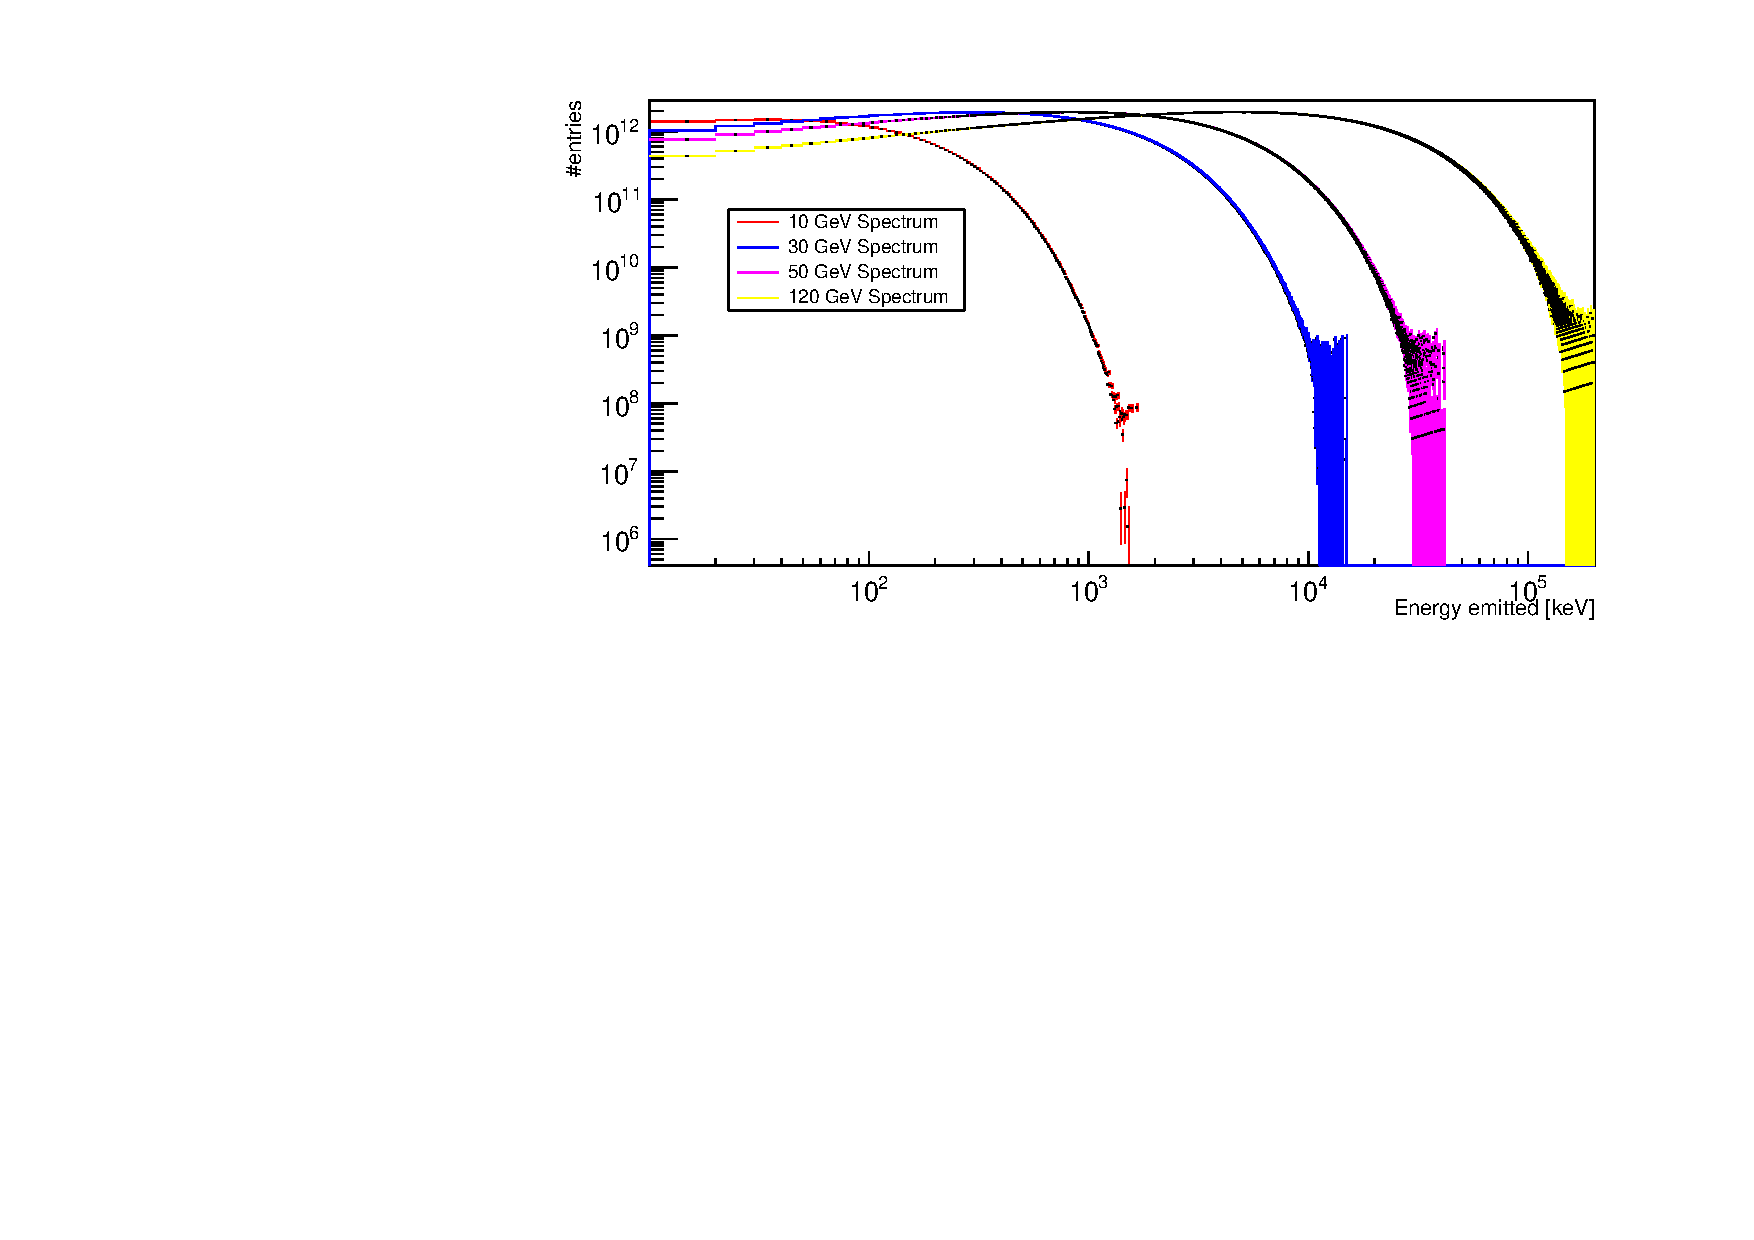
\includegraphics[width=\textwidth,height=0.55\textwidth]{\appdirb/syn_spectra.pdf}
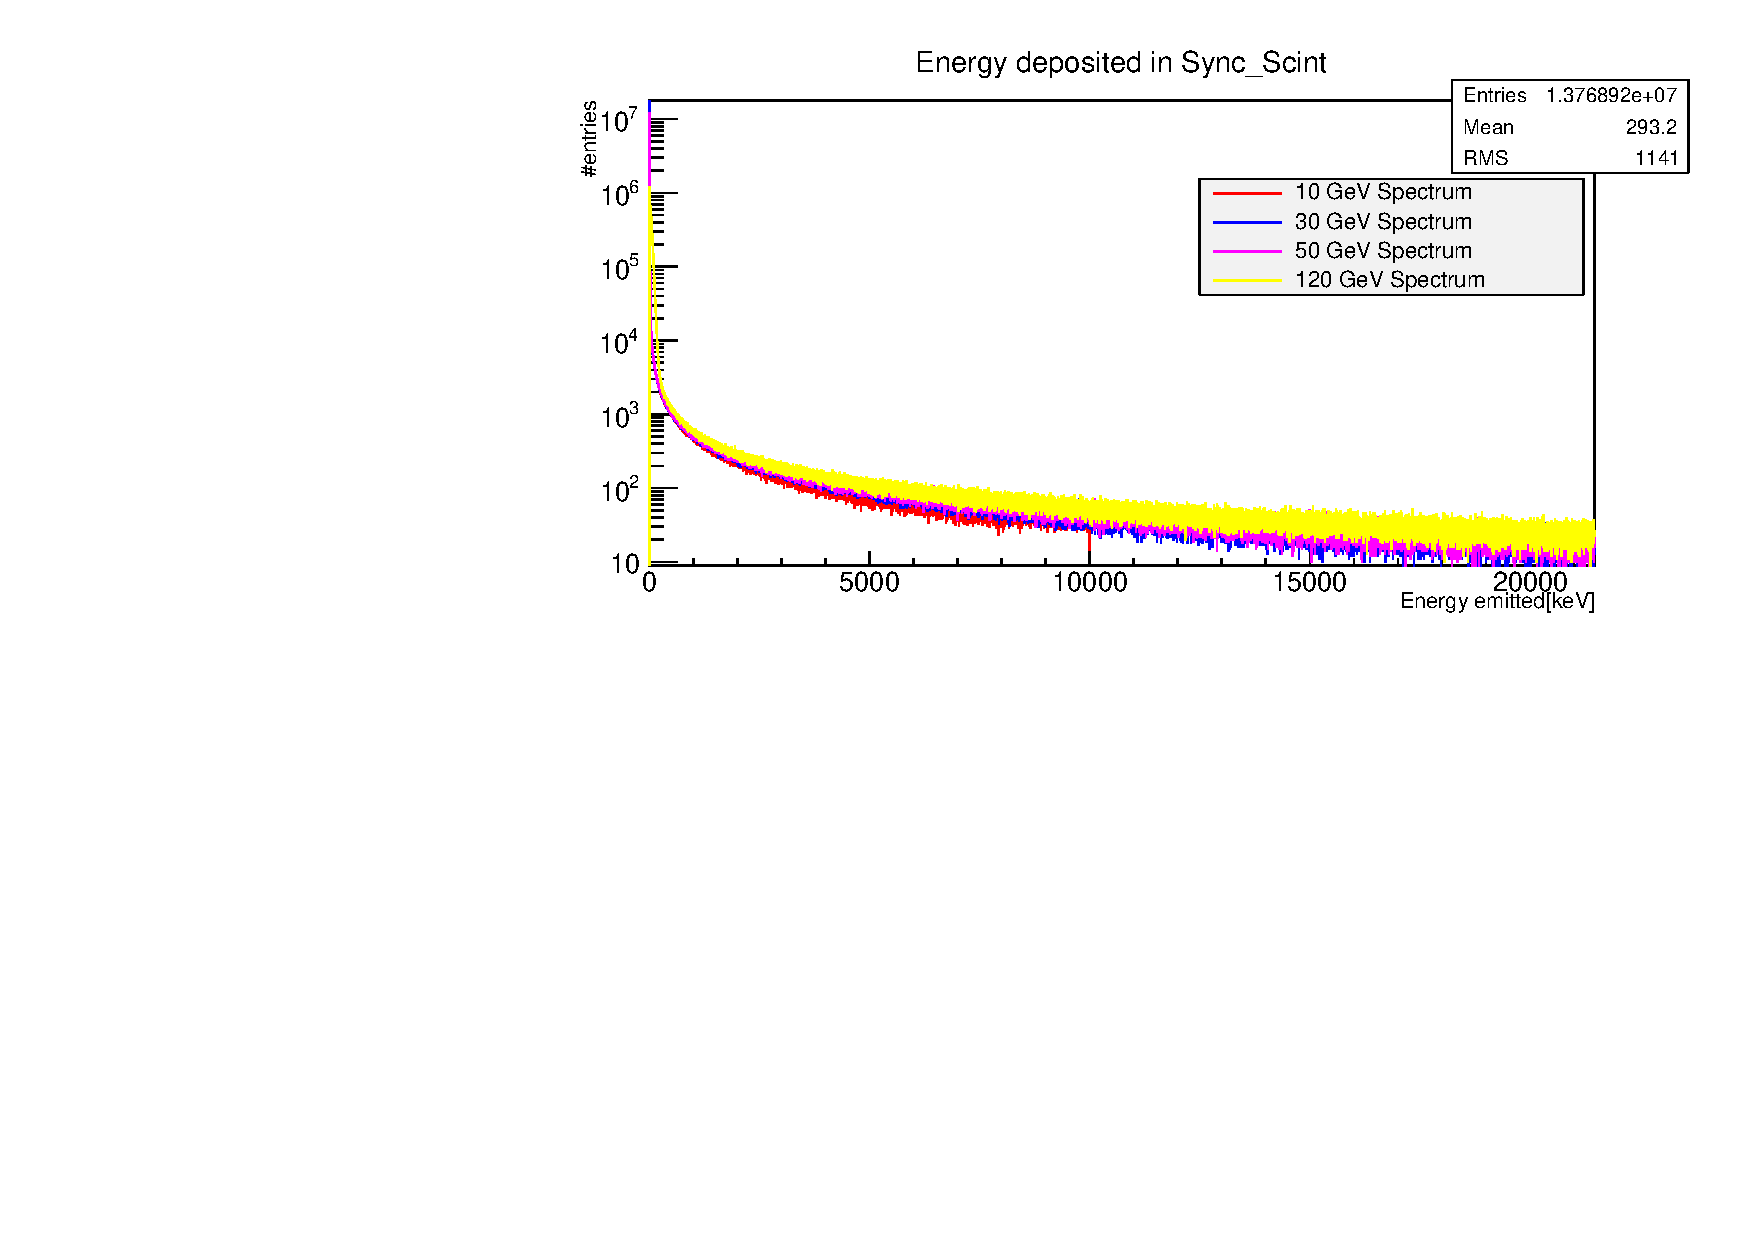
\includegraphics[width=\textwidth,height=0.55\textwidth]{\appdirb/brems_spectra.pdf}
\caption{upper plot: Spectrum for a single synchrotron photon emitted by an electron in the MC simulation. \\
Bottom plot: total energy deposited in the BGO for one electron event after the bremsstrahlung is included in the simulation.}
\label{fig:synch_spectrum}
\end{figure}

\section{Shower profile}
\label{appB:sec:shower-profile}

\subsection{Electromagnetic shower}
\label{appB:sec:shower-profile-ecal}

\subsection{Hadronic shower}
\label{appB:sec:shower-profile-hcal}

%%% Local Variables:
%%% mode: latex
%%% TeX-master: "../PhDthesis"
%%% End:
